\documentclass{article}\usepackage[]{graphicx}\usepackage[]{color}
%% maxwidth is the original width if it is less than linewidth
%% otherwise use linewidth (to make sure the graphics do not exceed the margin)
\makeatletter
\def\maxwidth{ %
  \ifdim\Gin@nat@width>\linewidth
    \linewidth
  \else
    \Gin@nat@width
  \fi
}
\makeatother

\definecolor{fgcolor}{rgb}{0.345, 0.345, 0.345}
\newcommand{\hlnum}[1]{\textcolor[rgb]{0.686,0.059,0.569}{#1}}%
\newcommand{\hlstr}[1]{\textcolor[rgb]{0.192,0.494,0.8}{#1}}%
\newcommand{\hlcom}[1]{\textcolor[rgb]{0.678,0.584,0.686}{\textit{#1}}}%
\newcommand{\hlopt}[1]{\textcolor[rgb]{0,0,0}{#1}}%
\newcommand{\hlstd}[1]{\textcolor[rgb]{0.345,0.345,0.345}{#1}}%
\newcommand{\hlkwa}[1]{\textcolor[rgb]{0.161,0.373,0.58}{\textbf{#1}}}%
\newcommand{\hlkwb}[1]{\textcolor[rgb]{0.69,0.353,0.396}{#1}}%
\newcommand{\hlkwc}[1]{\textcolor[rgb]{0.333,0.667,0.333}{#1}}%
\newcommand{\hlkwd}[1]{\textcolor[rgb]{0.737,0.353,0.396}{\textbf{#1}}}%

\usepackage{framed}
\makeatletter
\newenvironment{kframe}{%
 \def\at@end@of@kframe{}%
 \ifinner\ifhmode%
  \def\at@end@of@kframe{\end{minipage}}%
  \begin{minipage}{\columnwidth}%
 \fi\fi%
 \def\FrameCommand##1{\hskip\@totalleftmargin \hskip-\fboxsep
 \colorbox{shadecolor}{##1}\hskip-\fboxsep
     % There is no \\@totalrightmargin, so:
     \hskip-\linewidth \hskip-\@totalleftmargin \hskip\columnwidth}%
 \MakeFramed {\advance\hsize-\width
   \@totalleftmargin\z@ \linewidth\hsize
   \@setminipage}}%
 {\par\unskip\endMakeFramed%
 \at@end@of@kframe}
\makeatother

\definecolor{shadecolor}{rgb}{.97, .97, .97}
\definecolor{messagecolor}{rgb}{0, 0, 0}
\definecolor{warningcolor}{rgb}{1, 0, 1}
\definecolor{errorcolor}{rgb}{1, 0, 0}
\newenvironment{knitrout}{}{} % an empty environment to be redefined in TeX

\usepackage{alltt}[14pt]
\usepackage{amsmath}
\usepackage{amsfonts}
\usepackage{amssymb}
\usepackage{hyperref}
\usepackage{url}
\usepackage{booktabs}
\usepackage{graphicx}
\usepackage[margin=3cm]{geometry}
\usepackage[tight,TABTOPCAP]{subfigure}


\title{Beetle Phylogeny}
\author{Zachary Foster}
\date{\today}



\IfFileExists{upquote.sty}{\usepackage{upquote}}{}

\begin{document}

\maketitle



\section{Analytical Methods}
Sequences of the ribosomal 18S subunit and the \textit{Wingless} gene were used to infer the phylogeny of 28 species of beetle, representing multiple suborders. Mesquite \cite{maddison_mesquite:_2001} and Paup \cite{swofford_paup*._2003} were used to conduct parsimony and maximum-likelihood analysis on both sets of sequences.

\subsection*{Multiple Sequence Alignment}
Alignment of DNA and protein sequence was done using Mafft on the "L-INS-i" setting for high accuracy alignments. 
DNA alignments for the \textit{Wingless} gene sequence was obtained by mapping the DNA sequences to the protein alignment in Mesquite. 

\subsection*{Tree Inference}
Parsimony analysis and bootstrapping was done with Paup using default settings, with 1000 bootstrap replicates used. 
In the maximum-likelihood analysis, a proportion of invariant sites following a gamma distribution was assumed and the gamma shape parameter was estimated during tree search. 
The default settings were used for the bootstrapping analysis due to computing restrictions.
Maximum likelihood bootstrapping was done in Paup as well and 100 bootstrap replicates were used. 



\section{Results}
The phylogeny inferred using the 18S ribosomal sequence was much more resolved than the phylogeny inferred from the \textit{Wingless} gene sequence and roughly corresponded to specimen classification. 
The four analysis methods used for each sequence has similar results(Figures~\ref{fig:18s} and ~\ref{fig:wingless}). 

\subsection*{18S Phylogeny}
The phylogeny of 18S is well resolved and monophyletic clades mostly correspond to beetle suborders.
In the best maximum-likelihood tree, half of the Geadephaga species occurs within the Hydradephaga clade, possibly due to short branch lengths at the base of the clade. The maximum-likelihood bootstrap method and both parsimony analyses show Geadephaga and Hydradephaga as separate monophyletic clades.
Polytomies in Geadephaga and Hydradephaga (Figure \ref{fig:18s} \subref{fig:18s_maximum_liklihood_100_bootstrap} and \subref{fig:18s_parsimony_1000-bootstrap}) represent uncertain placement of species within the suborder. 

\subsection*{\textit{Wingless} Phylogeny}
The phylogeny inferred using the \textit{Wingless} gene sequence was much less resolved than that of 18S.
The only monophyletic group inferred was Geadephaga in the maximum-likelihood analysis in which invariant sites were simulated.
The bootstrap analysis using both parsimony and maximum-likelihood techniques yielded similar, but unresolved results. 

\begin{figure}[ht]
 \centering
 \subfigure[Strict consensus tree of 2 top-scoring trees using maximum-likelihood]{
  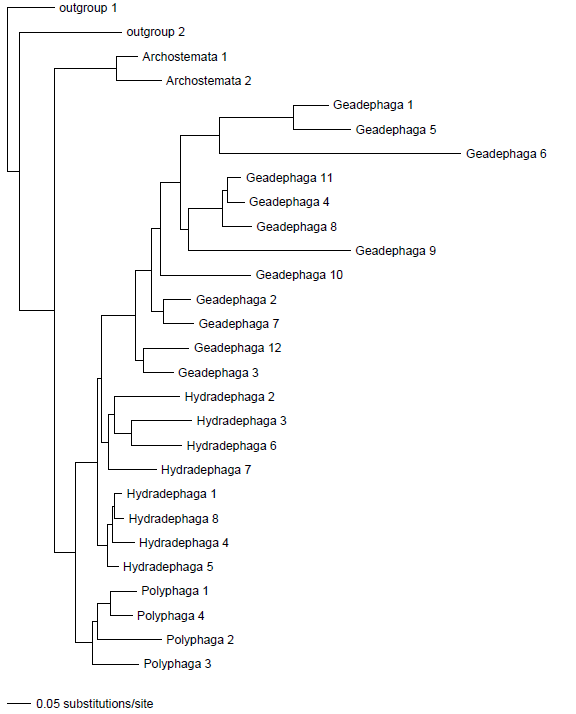
\includegraphics[height=9cm]{18s_maximum_liklihood}
   \label{fig:18s_maximum_liklihood}
   }
 \hspace{10pt}
 \subfigure[Majority-rule consensus tree of 100 maximum- likelihood bootstrap replicates]{
  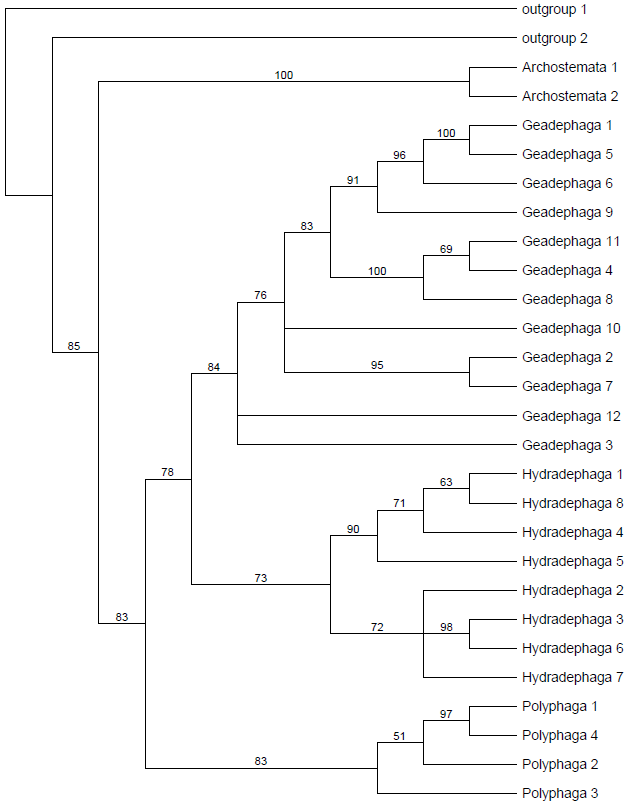
\includegraphics[height=9cm]{18s_maximum_liklihood_100_bootstrap}
   \label{fig:18s_maximum_liklihood_100_bootstrap}
   }

 \subfigure[Strict consensus tree of 4 top-scoring trees using parsimony. Tree Length = 2136.]{
  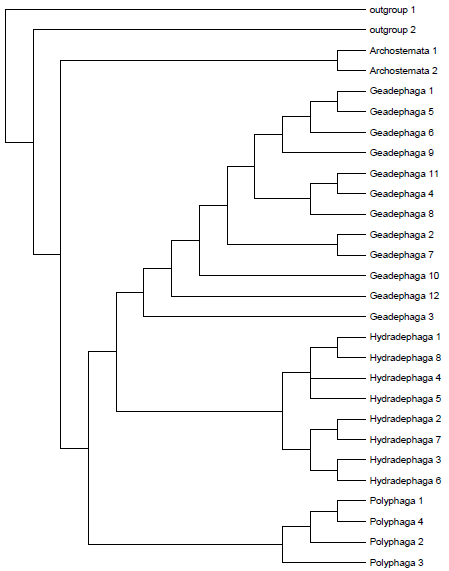
\includegraphics[height=9cm]{18s_parsimony_consensus}
   \label{fig:18s_parsimony_consensus}
   }
 \hspace{10pt}   
 \subfigure[Majority-rule consensus tree of 1000 parsimony bootstrap replicates]{
  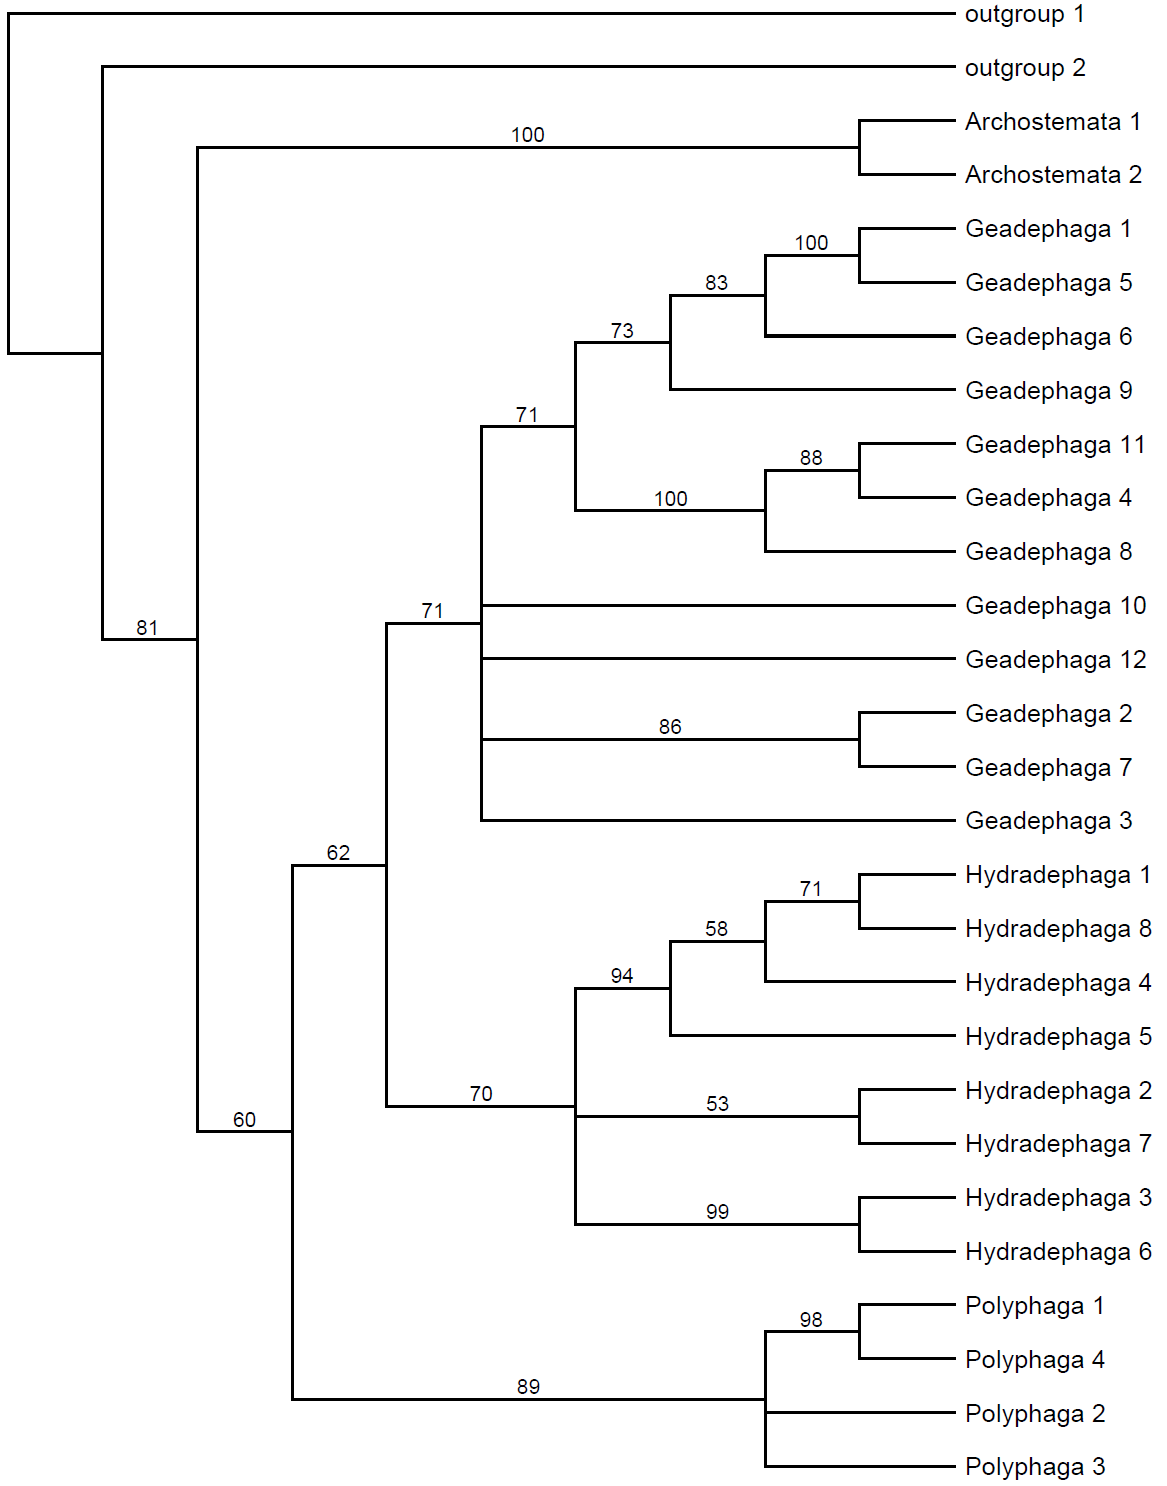
\includegraphics[height=9cm]{18s_parsimony_1000-bootstrap}
   \label{fig:18s_parsimony_1000-bootstrap}
   }
 \caption[fig:18s]{%
  Results of phylogeny inference using the 18S ribosomal gene sequence. 
  Paup and Mesquite were used with default settings unless otherwise noted. 
  The best scoring maximum-likelihood tree \subref{fig:18s_maximum_liklihood} was determined by estimating the gamma shape parameter for proportion of invariant site during the tree search.
  286 informative characters were used in the analysis.}
 \label{fig:18s}
\end{figure}


\begin{figure}[ht]
 \centering
 \subfigure[Top-scoring tree using maximum- likelihood. The value of the gamma shape parameter for proportion of invariable sites was inferred during tree search.]{
  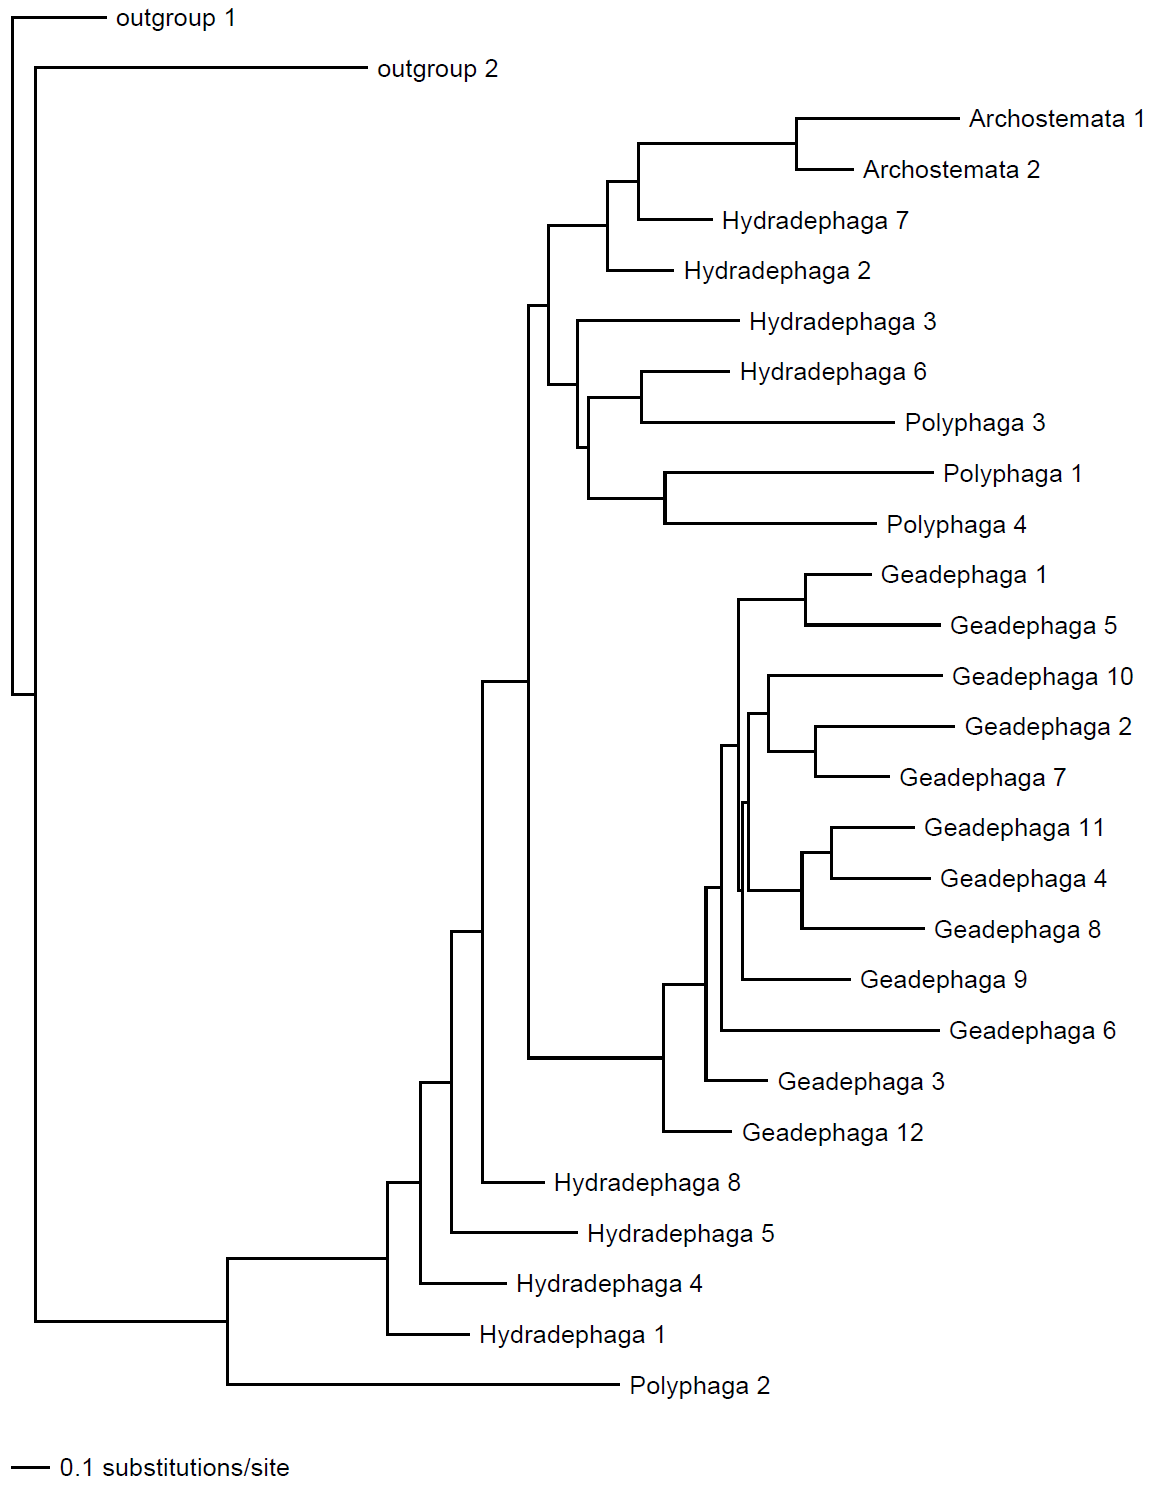
\includegraphics[height=9cm]{protein_maximum-liklihood_best}
   \label{fig:protein_maximum-liklihood_best}
   }
 \hspace{10pt}
 \subfigure[Majority-rule consensus tree of 100 maximum- likelihood bootstrap replicates]{
  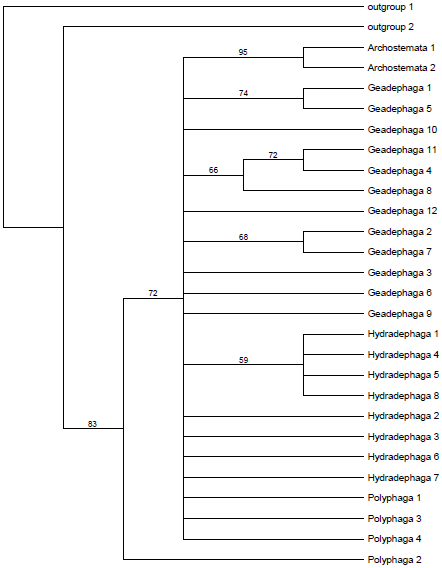
\includegraphics[height=9cm]{protein_maximum-liklihood_bootstrap}
   \label{fig:protein_maximum-liklihood_bootstrap}
   }

 \subfigure[Strict consensus tree of 4 top-scoring trees using parsimony. Tree Length = 2136.]{
  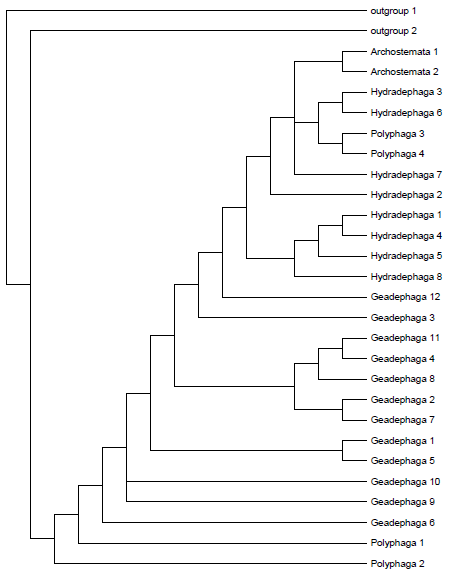
\includegraphics[height=9cm]{protein_parsimony_consensus}
   \label{fig:protein_parsimony_consensus}
   }
 \hspace{10pt}   
 \subfigure[Majority-rule consensus tree of 1000 parsimony bootstrap replicates]{
  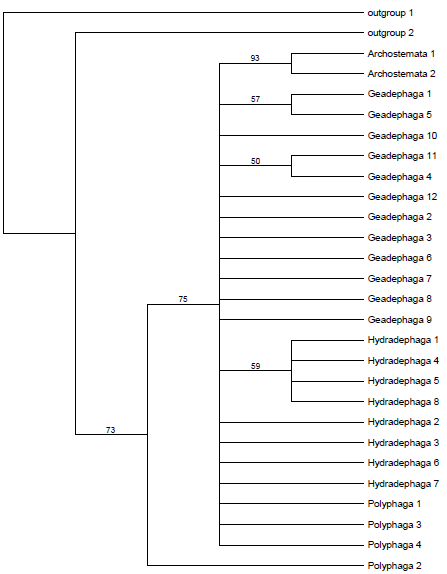
\includegraphics[height=9cm]{protein_parsimony_1000-bootstrap}
   \label{fig:protein_parsimony_1000-bootstrap}
   }
 \caption[fig:wingless]{%
  Results of phylogeny inference using the \textit{Wingless} gene sequence. 
  Paup and Mesquite were used with default settings unless otherwise noted. 
  The best scoring maximum- likelihood tree \subref{fig:protein_maximum-liklihood_best} was determined by estimating the gamma shape parameter for proportion of invariant site during the tree search.
  286 informative characters were used in the analysis.}
 \label{fig:wingless}
\end{figure}

\bibliographystyle{plain}
\bibliography{../references}

\end{document}
